\chapter{Case Study}
\label{ch:case_study}

In this case study, we analyze a couple of real projects, hosted on GitHub, to get a better understanding of DDU.
More specifically, we are interested in how DDU is affected by different kinds of tests, e.g. unit tests and integration tests, and testing techniques like parameterized testing.
Essentially, we are interested in finding testing approaches that improve the diagnosability.
This knowledge could be used to guide developers in writing tests during the software development process.

% First, we discuss the selection criteria that are used for selecting open source projects to analyze.
% Secondly, we explain the approach for analyzing the impact of different kinds of tests on DDU.
% Then, for each individual term of DDU, i.e. normalized density, diversity, and uniqueness, we give examples to clarify how the term changes with regard to related tests.
% Subsequently, we discuss the DDU metric as a whole.
% Finally, we conclude this case study with observations and recommendations.
First, we describe the approach used for this case study and the selection criteria. Then, we explore how DDU and its individual components vary as a consequence to types of tests. 


\section{Approach}

To get a better understanding of how DDU varies as a consequence to testing, we use \texttt{ddu-maven-plugin}\footnote{\url{https://github.com/aperez/ddu-maven-plugin}}, written by Perez, to instrument Java code and construct the activity matrix.
Once we obtain the activity matrices, we analyze the data using multiple Python scripts\footnote{\url{https://github.com/aaronang/ddu}}.
With these two tools we collect data such as number of tests, number of components, density, normalized density, diversity, uniqueness, DDU, and the activity matrix.

Then, we analyze the collected data and show examples that illustrate how DDU and its individual terms vary as a consequence to particular kinds of tests.
We are interested in what kinds of testing approaches result in a high or low DDU value.

Note that \texttt{ddu-maven-plugin} is able to instrument the code for three different granularity levels, namely statements, branches, and methods.
By default \texttt{ddu-maven\-plugin} uses the method level granularity.
In this study, we make use of the method level granularity because it keeps the activity matrices compact and therefore easier to discuss.
In \autoref{fig:hist_method_branch}, we observe that the DDU distribution for branch level and method level granularity are following a similar trend.

\begin{figure}
    \centering
    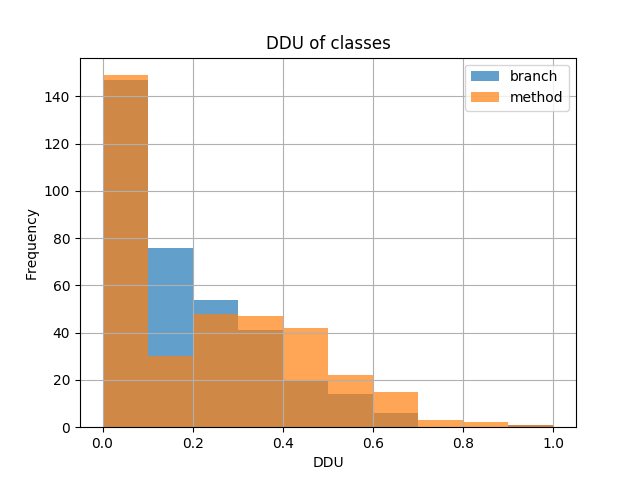
\includegraphics[width=\linewidth]{figures/histogram_ddu_method_branch}
    \caption{DDU distribution comparison between branch level and method level granularity.}
    \label{fig:hist_method_branch}
\end{figure}


\section{Selection}

The selection of open source projects is done according to the following criteria.

\emph{The project must have a executable test suite.}
To compute the DDU for a software project, we must construct an activity matrix, also known as program spectra.
The program spectra is constructed by running the test suite and instrumenting the code such that we can keep track of what parts of the code are executed during a program execution.

\emph{The project must use Apache Maven, a software project management and comprehension tool.}
The current tool that instruments the code to construct the activity matrix is implemented as a Maven plugin. Note that the current Maven plugin does not work for all Maven projects, and therefore only projects, that can be analyzed with this plugin, are used.

% \begin{itemize}
%     \item The project must have a executable test suite.
    
%     To compute the DDU for a software project, we must construct an activity matrix, also known as program spectra.
%     The program spectra is constructed by running the test suite and instrumenting the code such that we can keep track of what parts of the code are executed during a program execution.
    
%     \item The project must use Apache Maven, a software project management and comprehension tool.
    
%     The current tool that instruments the code to construct the activity matrix is implemented as a Maven plugin. Note that the current Maven plugin does not work for all Maven projects, and therefore only projects, that can be analyzed with this plugin, are used.
% \end{itemize}

Based on these requirements, we choose the following open source projects.

\begin{itemize}[noitemsep]
    \item Commons CSV\footnote{\url{https://github.com/apache/commons-csv}}: a library that provides a simple interface for reading and writing CSV files of various types.
    \item Commons Text\footnote{\url{https://github.com/apache/commons-text}}: a library focused on algorithms working on strings.
    \item Commons IO\footnote{\url{https://github.com/apache/commons-io}}: a library of utilities to assist with developing IO functionality.
    \item Guice\footnote{\url{https://github.com/google/guice}}: a lightweight dependency injection framework for Java 6 and above.
    \item Jsoup\footnote{\url{https://github.com/jhy/jsoup}}: an API for extracting and manipulating data, using the best of DOM, CSS, and jquery-like methods.
\end{itemize}



\section{Normalized Density}

In \autoref{fig:hist_normalized_density}, we show the distribution of normalized densities for all classes of the five open source projects mentioned before.
The average equals to 0.5145.
The peak for the interval [0, 0.1] is primarily caused by classes that are exercised by test cases that involve all components.
47 classes in the interval [0, 0.1] consist of only one method.
A class with one method will always have a density of 1.0 and therefore a normalized density of 0.
    
\begin{figure}
    \centering
    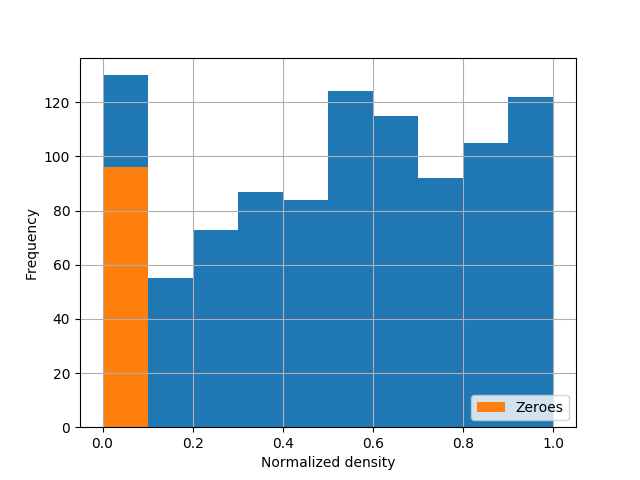
\includegraphics[width=\linewidth]{figures/histogram_normalized_density}
    \caption{Normalized density distribution.}
    \label{fig:hist_normalized_density}
\end{figure}

The normalized density value is low when a class is tested by many tests that only cover a couple of methods. 
For example, \texttt{org.apache.commons.csv.CSVRecord} has 17 methods (excluding its constructors) and its spectra looks as follows.
Note that not all transactions that hit \texttt{CSVRecord} methods are shown, but in the case of \texttt{CSVRecord}, all its transactions look similar; each transaction only hits a couple of components.


\begin{table}[]
\scriptsize
\centering
\caption{Partial activity matrix of the \texttt{CSVRecord} class.}
\label{tab:csvrecordtest}
\noindent\makebox[\textwidth]{%
\begin{tabular}{l|l|l|l|l|l|l|l|l|l|l|l|l|l|l|l|l|l}
transaction & $c_1$ & \multicolumn{15}{c|}{\dots} & $c_{17}$\\ \hline
\texttt{CSVRecordTest\#testGetStringNoHeader} & 1 & 0 & 0 & 0 & 0 & 0 & 0 & 0 & 0 & 0 & 0 & 0 & 0 & 0 & 0 & 0 & 0        \\ \hline
\texttt{CSVRecordTest\#testGetUnmappedPositiveInt} & 0 & 0 & 0 & 0 & 0 & 0 & 0 & 0 & 0 & 0 & 1 & 0 & 0 & 0 & 0 & 0 & 0   \\ \hline
\texttt{CSVRecordTest\#testGetUnmappedNegativeInt} & 0 & 0 & 0 & 0 & 0 & 0 & 0 & 0 & 0 & 0 & 1 & 0 & 0 & 0 & 0 & 0 & 0   \\ \hline
\texttt{CSVRecordTest\#testGetUnmappedEnum} & 1 & 0 & 0 & 0 & 0 & 0 & 0 & 0 & 0 & 0 & 0 & 0 & 0 & 1 & 0 & 0 & 0          \\ \hline
\texttt{CSVRecordTest\#testGetUnmappedName} & 1 & 0 & 0 & 0 & 0 & 0 & 0 & 0 & 0 & 0 & 0 & 0 & 0 & 0 & 0 & 0 & 0         
\end{tabular}}
\end{table}


In the partial spectra of \texttt{CSVRecord} shown above, the columns are the methods of \texttt{CSVRecord}.
So, for example, in the first row, we observe that the transaction \texttt{testGetStringNoHeader} only hits one method, indicated by a 1.
The normalized density of \texttt{CSVRecord} is low because its test cases only cover a couple components and this causes the activity matrix to become sparse.
Thus, the more components a class has, the greater the impact of a test, that hits a relative small number of components, has on the sparseness of the activity matrix.

\begin{table}[]
\scriptsize
\centering
\caption{Partial activity matrix of the \texttt{ConstructorInjectorStore} class.}
\label{my-label}
\noindent\makebox[\textwidth]{%
\begin{tabular}{l|l|l|l|l|l|l}
transaction                                    & $c_1$ & \multicolumn{4}{c|}{\dots} & $c_6$ \\ \hline
\texttt{ImplicitBindingTest\#testDefaultImplementation}  & 1    & 0    & 1    & 1    & 1    & 1    \\ \hline
\texttt{ImplicitBindingTest\#testProvidedByNonEmptyEnum} & 1    & 0    & 1    & 1    & 1    & 1    \\ \hline
\texttt{ImplicitBindingTest\#testDefaultProvider}        & 1    & 0    & 1    & 1    & 1    & 1    \\ \hline
\texttt{ImplicitBindingTest\#testProvidedByEmptyEnum}    & 1    & 0    & 1    & 1    & 1    & 1    \\ \hline
\texttt{ImplicitBindingTest\#testImplicitJdkBindings}    & 1    & 0    & 1    & 1    & 1    & 1   
\end{tabular}}
\end{table}

In the partial spectra of \texttt{com.google.inject.internal.Constructor\-Injector\-Store}, a Guice class, shown above, we observe a high density; almost all methods of \texttt{Constructor\-Injector\-Store} are hit in every single test.
Since the density is high: 0.8351, the normalized density is low: 0.3298.

So, ideally, to obtain a high value for the normalized density, we need a good balance between tests that cover many components and tests that cover a few.
In Commons Text, the \texttt{org.apache.commons.text.beta.StrLookup} class has a normalized density of 0.9512.
In the partial spectra, shown below, we observe that each test case covers 50\% of the components and therefore this particular class obtains a density close to 0.5 and a normalized density close 1.0.

\begin{table}[]
\scriptsize
\centering
\caption{My caption}
\label{my-label}
\noindent\makebox[\textwidth]{%
\begin{tabular}{l|l|l|l|l}
transaction                                                 & $c_1$ & \multicolumn{2}{c|}{\dots} & $c_4$ \\ \hline
\texttt{StrLookupTest\#testNoneLookup}                               & 0    & 1           & 0           & 1    \\ \hline
\texttt{StrLookupTest\#testSystemPropertiesLookupReplacedProperties} & 1    & 1           & 0           & 0    \\ \hline
\texttt{StrLookupTest\#testSystemPropertiesLookupUpdatedProperty}    & 1    & 1           & 0           & 0    \\ \hline
\texttt{StrLookupTest\#testMapLookup\_nullMap}                       & 0    & 1           & 1           & 0    \\ \hline
\texttt{StrLookupTest\#testMapLookup}                                & 0    & 1           & 1           & 0   
\end{tabular}}
\end{table}

In short, to obtain a good value for normalized density, we could suggest the developer to write tests that either cover many components, a few, or something in between based on the density.
If the density is lower than `0.5`, we could suggest the developer to write tests that cover many components.
If the density is higher than `0.5`, we could suggest the developer to write tests that cover a few components.
Either way, suggesting the developer to write tests that cover a certain number of components is probably not practical.


\section{Diversity}

In \autoref{fig:histogram_diversity}, the distribution of diversity of classes is shown.
The average is 0.4813.
The peak for the interval [0, 0.1] occurs for various reasons.
The first reason is that there are classes with only one method and therefore every row is identical, resulting in a diversity of 0.
The second reason is that for some classes there exist only one test case, and in the current Python script the diversity defaults to 0 when there is only one test case.
The third reason is that some classes only have test cases that have identical activity patterns.

\begin{figure}
    \centering
    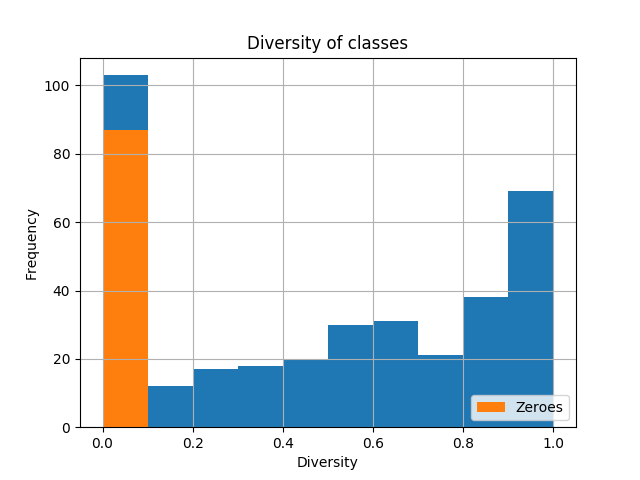
\includegraphics[width=\linewidth]{figures/histogram_diversity}
    \caption{Diversity distribution}
    \label{fig:histogram_diversity}
\end{figure}

Intuitively, the diversity has a low value when the number of identical transactions, i.e. identical rows in the activity matrix, is high.
Vice versa, the diversity is high when the number of identical transaction activity is low.

\begin{table}[]
\scriptsize
\centering
\caption{My caption}
\label{my-label}
\noindent\makebox[\textwidth]{%
\begin{tabular}{l|l|l|l|l}
transaction                    & $c_1$ & \multicolumn{2}{c|}{\dots} & $c_4$ \\ \hline
\texttt{ElementTest\#testCssPath}       & 1  & 0         & 1         & 0  \\ \hline
\texttt{ElementTest\#testSetHtmlTitle}  & 0  & 0         & 1         & 0  \\ \hline
\texttt{ElementTest\#moveByAppend}      & 0  & 0         & 1         & 0  \\ \hline
\texttt{ElementTest\#testClassUpdates}  & 0  & 0         & 1         & 0  \\ \hline
\texttt{ElementTest\#testAddNewElement} & 0  & 0         & 1         & 0  
\end{tabular}}
\end{table}

In the partial spectra of \texttt{org.jsoup.select.Evaluator} of Jsoup shown above, we observe that almost every transaction has an identical activity and therefore the diversity is low: 0.0901.
Another reason for the low diversity of \texttt{org.jsoup.select.Evaluator} is that it is covered by 277 test cases, while there are only $2^4 = 16$ possible different test cases.
After 16 unique test cases every additional test case will have a negative effect on the diversity because it will share similar activity with an existing test case.

\begin{table}[]
\scriptsize
\centering
\caption{My caption}
\label{my-label}
\noindent\makebox[\textwidth]{%
\begin{tabular}{l|l|l|l|l|l|l|l|l|l|l}
transaction                                                                     & $c_1$ & \multicolumn{8}{c|}{\dots}         & $c_{10}$ \\ \hline
\texttt{MembersInjectorTest\#testMembersInjectorFromBinder}                              & 1    & 1 & 1 & 1 & 0 & 0 & 1 & 1 & 1 & 1     \\ \hline
\texttt{ElementApplyToTest\#testGetMembersInjector}                                      & 1    & 1 & 1 & 1 & 1 & 1 & 1 & 1 & 1 & 0     \\ \hline
\texttt{ElementApplyToTest\#testElementInitialization}                                   & 1    & 1 & 1 & 1 & 0 & 1 & 0 & 1 & 1 & 0     \\ \hline
\texttt{ElementsTest\#testGetMembersInjector}                                            & 1    & 1 & 1 & 0 & 1 & 0 & 1 & 1 & 1 & 0     \\ \hline
\texttt{ElementsTest\#testElementInitialization}                                         & 1    & 1 & 1 & 1 & 0 & 0 & 0 & 1 & 1 & 0     \\ \hline
\texttt{TypeListenerTest\#testLookupsAtInjectorCreateTime}                               & 1    & 1 & 1 & 1 & 0 & 0 & 1 & 1 & 1 & 0     \\ \hline
\texttt{TypeListenerTest\#testConstructedTypeListenerIs\dots} & 0    & 1 & 0 & 1 & 0 & 0 & 1 & 1 & 1 & 0     \\ \hline
\texttt{TypeListenerTest\#testInjectMembersTypeListenerFails}                            & 0    & 1 & 0 & 0 & 0 & 0 & 1 & 1 & 1 & 0     \\ \hline
\texttt{NoopOverrideTest\#testGetMembersInjector}                                        & 1    & 1 & 1 & 1 & 1 & 1 & 1 & 1 & 1 & 0     \\ \hline
\texttt{NoopOverrideTest\#testElementInitialization}                                     & 1    & 1 & 1 & 1 & 0 & 1 & 0 & 1 & 1 & 0    
\end{tabular}}
\end{table}

In the activity matrix of \texttt{com.google.inject.spi.MembersInjectorLookup}, a Guice class, shown above, we observe that almost every transaction has a unique activity and therefore its diversity is high.
Note that the diversity suffers when there are too many test cases, but does not suffer from a low number of test cases, i.e. a high diversity can be obtained with a couple unique system transactions.

\begin{table}[]
\scriptsize
\centering
\caption{My caption}
\label{my-label}
\noindent\makebox[\textwidth]{%
\begin{tabular}{l|l|l|l|l|l}
transaction                                       & $c_1$ & \multicolumn{3}{c|}{\dots} & $c_5$ \\ \hline
\texttt{ParameterizedLevenshteinDistanceTest\#test[0]} & 0    & 1       & 1       & 0      & 0    \\ \hline
\texttt{ParameterizedLevenshteinDistanceTest\#test[1]} & 0    & 1       & 1       & 0      & 0    \\ \hline
\texttt{ParameterizedLevenshteinDistanceTest\#test[2]} & 0    & 1       & 1       & 0      & 0    \\ \hline
\texttt{ParameterizedLevenshteinDistanceTest\#test[3]} & 0    & 1       & 1       & 0      & 0    \\ \hline
\texttt{ParameterizedLevenshteinDistanceTest\#test[4]} & 0    & 1       & 1       & 0      & 0    \\ \hline
\texttt{ParameterizedLevenshteinDistanceTest\#test[5]} & 0    & 1       & 1       & 0      & 0    \\ \hline
\texttt{ParameterizedLevenshteinDistanceTest\#test[6]} & 0    & 1       & 1       & 0      & 0    \\ \hline
\texttt{ParameterizedLevenshteinDistanceTest\#test[7]} & 0    & 1       & 1       & 0      & 0    \\ \hline
\texttt{ParameterizedLevenshteinDistanceTest\#test[8]} & 0    & 1       & 1       & 0      & 0   
\end{tabular}}
\end{table}

An interesting case for diversity is parameterized testing, shown in the partial spectra above.
The \texttt{LevenshteinDistance} spectra consists primarily of parameterized test and has a diversity of 0.3167.
Although parameterized is a common practice to test different inputs for a unit, it has a negative effect on the diversity due to identical activity patterns.


\section{Uniqueness}

In the figure below, the distribution of uniqueness of classes are shown.
The average is 0.7696.

\begin{figure}
    \centering
    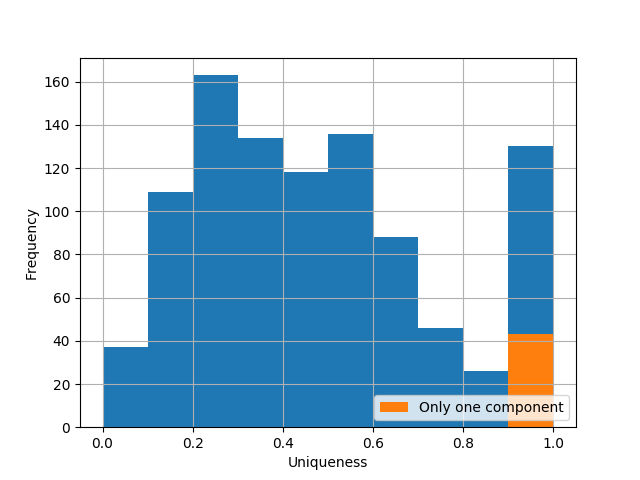
\includegraphics[width=\linewidth]{figures/histogram_uniqueness}
    \caption{Distribution of uniqueness.}
    \label{fig:uniqueness}
\end{figure}

The peak for the interval [0.9, 1.0] is partially caused by classes that only have one component; activity matrices that consist of one component always have a uniqueness of 1.0.
More specifically, there are 130 classes that have a uniqueness of 1.0 and 47 out of the 130 only have one component.

\begin{table}[]
\scriptsize
\centering
\caption{My caption}
\label{my-label}
\noindent\makebox[\textwidth]{%
\begin{tabular}{l|l|l|l|l|l|l|l|l|l|l|l|l}
transaction                                            & $c_1$ & \multicolumn{10}{c|}{\dots}           & $c_{12}$ \\ \hline
\texttt{CopyUtilsTest\#testCopy\_byteArrayToWriterWithEncoding} & 0     & 0 & 1 & 0 & 0 & 1 & 0 & 0 & 0 & 0 & 1 & 0        \\ \hline
\texttt{CopyUtilsTest\#copy\_stringToOutputStream}              & 0     & 0 & 0 & 0 & 0 & 0 & 0 & 0 & 0 & 0 & 1 & 1        \\ \hline
\texttt{CopyUtilsTest\#testCopy\_readerToOutputStream}          & 0     & 0 & 0 & 0 & 0 & 0 & 0 & 0 & 1 & 0 & 1 & 0        \\ \hline
\texttt{CopyUtilsTest\#copy\_readerToWriter}                    & 0     & 0 & 0 & 0 & 0 & 0 & 0 & 0 & 0 & 0 & 1 & 0        \\ \hline
\texttt{CopyUtilsTest\#copy\_byteArrayToWriter}                 & 0     & 1 & 0 & 0 & 0 & 0 & 0 & 0 & 0 & 1 & 1 & 0        \\ \hline
\texttt{CopyUtilsTest\#copy\_byteArrayToOutputStream}           & 0     & 0 & 0 & 0 & 1 & 0 & 0 & 0 & 0 & 0 & 0 & 0        \\ \hline
\texttt{CopyUtilsTest\#copy\_inputStreamToWriterWithEncoding}   & 0     & 0 & 1 & 0 & 0 & 0 & 0 & 0 & 0 & 0 & 1 & 0        \\ \hline
\texttt{CopyUtilsTest\#copy\_inputStreamToWriter}               & 0     & 1 & 0 & 0 & 0 & 0 & 0 & 0 & 0 & 0 & 1 & 0        \\ \hline
\texttt{CopyUtilsTest\#testCopy\_inputStreamToOutputStream}     & 0     & 0 & 0 & 0 & 0 & 0 & 1 & 0 & 0 & 0 & 0 & 0        \\ \hline
\texttt{CopyUtilsTest\#copy\_stringToWriter}                    & 1     & 0 & 0 & 0 & 0 & 0 & 0 & 0 & 0 & 0 & 0 & 0        \\ \hline
\texttt{IOUtilsTestCase\#testCopy\_String\_Writer}              & 1     & 0 & 0 & 0 & 0 & 0 & 0 & 0 & 0 & 0 & 0 & 0        \\ \hline
\texttt{IOUtilsTestCase\#testCopy\_ByteArray\_Writer}           & 0     & 1 & 0 & 0 & 0 & 0 & 0 & 0 & 0 & 1 & 1 & 0        \\ \hline
\texttt{IOUtilsTestCase\#testCopy\_ByteArray\_OutputStream}     & 0     & 0 & 0 & 0 & 1 & 0 & 0 & 0 & 0 & 0 & 0 & 0        \\ \hline
\texttt{IOUtilsTestCase\#testStringToOutputStream}              & 0     & 0 & 0 & 0 & 0 & 0 & 0 & 0 & 0 & 0 & 1 & 1       
\end{tabular}}
\end{table}

The uniqueness of an activity matrix is high when the number of unique columns is high.
For example, \texttt{org.apache.commons.io.CopyUtils} has a uniqueness of 0.9167, see spectra above.
This class has a high uniqueness because its test suite mostly consists of test cases that only cover a couple components each.

\begin{table}[]
\scriptsize
\centering
\caption{My caption}
\label{my-label}
\noindent\makebox[\textwidth]{%
\begin{tabular}{l|l|l|l|l|l|l|l}
transaction                                            & $c_1$ & \multicolumn{5}{c|}{\dots} & $c_7$ \\ \hline
\texttt{ReplacementsFinderTest\#testReplacementsHandler[1]} & 1     & 1   & 1   & 1   & 1   & 1  & 1     \\ \hline
\texttt{StringsComparatorTest\#testExecution}                   & 1     & 1   & 1   & 1   & 1   & 1  & 1     \\ \hline
\texttt{StringsComparatorTest\#testLongestCommonSubsequence}    & 1     & 1   & 1   & 1   & 1   & 1  & 1     \\ \hline
\texttt{StringsComparatorTest\#testLength}                      & 1     & 1   & 1   & 1   & 1   & 1  & 1    
\end{tabular}}
\end{table}

In the spectra above of \texttt{org.apache.commons.text.beta.diff.StringsComparator}, we observe that every component is covered in every transaction and therefore the uniqueness is low: 0.1429.
Although the matrix has no unique columns, its uniqueness is not 0.
So, to improve the uniqueness of this matrix, we could write tests that cover a few components each, resulting in each column being unique.

\section{DDU}

In the figure below, the distribution of DDU of classes are shown.
The average is 0.2264.

\begin{figure}
    \centering
    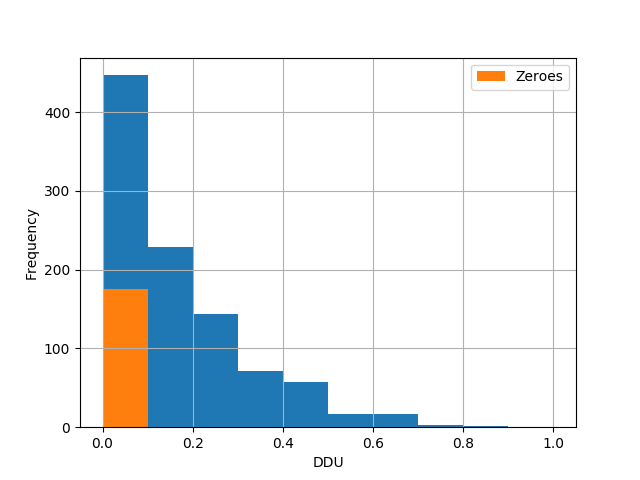
\includegraphics[width=\linewidth]{figures/histogram_ddu}
    \caption{DDU distribution.}
    \label{fig:my_label}
\end{figure}

Out of all the classes, there is only one class that has a DDU of 1.0, namely \texttt{org.apache.commons.io.output.BrokenOutputStream}, see spectra below.

\begin{table}[]
\scriptsize
\centering
\caption{My caption}
\label{my-label}
\noindent\makebox[\textwidth]{%
\begin{tabular}{l|l|l|l}
transaction                              & $c_1$ & $c_2$ & $c_3$ \\ \hline
\texttt{BrokenOutputStreamTest\#testClose}        & 0     & 0     & 1     \\ \hline
\texttt{BrokenOutputStreamTest\#testFlush}        & 0     & 1     & 0     \\ \hline
\texttt{BrokenOutputStreamTest\#testWrite}        & 1     & 0     & 0     \\ \hline
\texttt{TaggedOutputStreamTest\#testBrokenStream} & 1     & 1     & 1    
\end{tabular}}
\end{table}

Multiplying the individual terms might not be the right approach.

Based on the uniqueness observations, it seems that uniqueness at least requires the developer to write tests that cover a few components.
